%File: formatting-instruction.tex
\documentclass[letterpaper]{article}
\usepackage{flairs}%aaai
\usepackage{times}
\usepackage{helvet}
\usepackage{courier}
\usepackage{url}
% for figure grid
\usepackage{graphicx}
\graphicspath{ {figures/} }
\usepackage{caption}
\usepackage{subcaption}
\usepackage{wrapfig}
\usepackage{multirow}
\usepackage{tabularx}
\usepackage{paralist}
\usepackage{colortbl}
\usepackage{dingbat, pifont}
\definecolor{Gray}{gray}{0.9}

\usepackage{array} %for table fix width

\frenchspacing
\setlength{\pdfpagewidth}{8.5in}
\setlength{\pdfpageheight}{11in}
\pdfinfo{
/Title (Enhancing Linux Kernel Real-Time Performance through Centralized Timer Interrupt Handling)
/Author (Anonymous)}
\setcounter{secnumdepth}{0}  

\begin{document}
% This file is an adoption of the style file for AAAI Press 
% proceedings, working notes, and technical reports.  This file is made 
% with minimal changes by explicit permission from AAAI.
%
\title{Enhancing Linux Kernel Real-Time Performance through Centralized Timer Interrupt Handling}
\author{
\begin{tabular}{lllll}
  Zhouyi Zhou & Zhili Liu & Shancong Zhang & Jiemin Li & Dengke Du \\
  Mengke Sun  & Zhiqiang Wang & Hongyan Liu & Guoxin Xu & Yexin Han\\
%  & Dengke Du & Mengke Sun  & Zhiqiang Wang & Hongyan Liu & Guoxin Xu & Yexin Han\\
\end{tabular}
\\
Beijing UCAS Space Technology Co Ltd, Beijing, China\\
\{zhouyi.zhou, zhili.liu, sam.zhang, jiemin.li,
dengke.du, mengke.sun, zhiqiangwang, hongyan.liu,
xuguokai, hanyexin\}@ucas.com.cn\\ 
}

\maketitle

\begin{abstract}
In real-time and high-performance computing environments, predictable CPU behavior and low-
latency response are critical. The Linux kernel, by default, distributes periodic timer interrupts
(ticks) across all CPU cores, issues inter-processor interrupts (IPIs) and scheduling disturbances
that hinder deterministic performance. This paper investigates a method for improving Linux
kernel real-time behavior by centralizing timer interrupt handling and inter-processor interrupts
on periodically invoked function. We analyze the mechanism in detail, explain the interplay with
RCU context-tracking, and demonstrate the practical benefits both in a GPIO toggling environment
and a inter-processor communication environment. Our experiments show significant
improvements in interrupt latency and scheduling predictability, enabling more efficient real-time
and user-space networking applications. 
\end{abstract}


\section{Introduction}
Modern high-performance and real-time systems increasingly demand predictable CPU behavior,
low interrupt latency, and minimal system noise. However, general-purpose operating systems
like Linux are not originally designed with these strict requirements in mind. In particular, two key
sources of execution disturbance are periodic timer interrupts and inter-processor interrupts (IPIs)
— each of which independently contributes to unpredictability and jitter in CPU-bound workloads.
Timer Interrupts: The Linux kernel schedules periodic timer interrupts (commonly known as ticks)
on every CPU core to maintain kernel housekeeping, timekeeping, and scheduling. These
interrupts invoke routines for updating system time, triggering task rescheduling, handling timer
expiration, real time process bandwidth control, and advancing internal kernel mechanisms. For
typical workloads, such periodic processing is harmless or even necessary. However, for latency-
sensitive applications — such as user-space network packet processing, real-time control loops,
or audio/video pipelines — these timer interrupts pose significant interference by breaking
deterministic CPU execution.


While mechanisms like NOHZ\_FULL aim to reduce the frequency of such timer ticks, they cannot
completely eliminate them. Even in nohz\_full mode, the tick timer still fire periodically. Thus, strict
real-time applications still face residual interruptions even on nominally “isolated” cores.
Inter-Processor Interrupts (IPIs): In parallel with timer-related disturbances, IPIs represent another
major source of noise. IPIs are used in the kernel to coordinate state changes between cores —
for example, to trigger TLB shootdowns, wake remote tasks, or synchronize RCU grace periods.
From the perspective of an application pinned to a specific core, IPIs are unpredictable and
asynchronous, and can cause unwelcome preemption or context switches.
Although disabling timer interrupts may reduce local noise, it does not automatically prevent a
core from receiving IPIs initiated by other cores or subsystems. This means that even a core
exempt from ticks may still be interrupted arbitrarily due to kernel-wide coordination
mechanisms.


Our Approach: Full Isolation by timer bypass and IPI suppression. In this paper, we present a novel
and more aggressive approach to CPU isolation in Linux: We completely disable timer interrupt
processing on selected cores, ensuring no kernel tick-related activity occurs locally; We suppress
all non-essential inter-processor interrupts to those cores, using targeted kernel patches and
configuration to redirect such coordination elsewhere or delay it entirely. This level of isolation is
not achievable with existing mechanisms like NOHZ\_FULL or isolcpus alone. Our solution explicitly
separates time-related kernel responsibilities and reassigns them to maintenance mechanism,
which periodically execute the timer functionalities required for global correctness. Meanwhile,
isolated cores run continuously without being interrupted by either local timers or remote IPIs.
This approach is particularly effective in scenarios like GPIO toggling, where high precision and
low-latency response are critical, allowing the Linux isolation kernel to efficiently manage interrupts,
isolate processing on specific cores, and ensure that GPIO outputs are triggered in a timely manner,
free from interrupt interference or other system task disruptions.


\section{Related Work}\label{BG} 
\subsection{Timer Interrupt Control in the Linux Kernel}
The timer ticker design for Operating Systems has long exist before Linux kernel was
developed\cite{Corbet}.
The Linux kernel schedules periodic timer interrupts (ticks) on each CPU core for timekeeping,
process accounting, and scheduler activation. These interrupts are typically generated at (250 - 1K) Hz
and cause the kernel to preempt running tasks for internal maintenance.
To reduce this overhead, tickless systems were introduced. The NO\_HZ feature disables timer
interrupts on idle CPUs, and its extension, NOHZ\_FULL, attempts to eliminate ticks even during
user-space execution\cite{KernelDocNOHZ}. However, timer ticks still occur on NO\_HZ/NOHZ\_FULL CPUs because the
kernel want to do statistics works[3].
These mechanisms help reduce timer-induced jitter but do not eliminate all sources of latency.

\section{Methodology}\label{M}
Our proposed multimodal architecture amalgmates the visual, text and audio transformer encoders. The former two are adapted from Vanilla CLIP \cite{vanilla_clip} whereas the audio encoder is based on AudioCLIP \cite{audio_clip}. During training, all encoder layers of all modalities remain frozen, therefore retaining the model's pre-training knowledge while making it computationally efficient. To enhance the model's capability to be effective on the downstream task of video content moderation, prompt learning is enabled for the text and vision branches. We also introduce a fully-trainable projection layer at the end of the audio branch which learns the audio representations during training. Vanilla CLIP was tailored for the video input. We calculate the aggregate representations from both audio and vision branches.  The fused features along with the text features are then learned contrastively during training - maximizing the diagonal  (\textit{V$_{i}$},\textit{T$_{i}$}) of the cosine similarity matrix while minimizing other pairs of fused and text features. Maximizing the diagonal implies that the similarity score with the ground-truth class is maximized while others are minimized. The following sections discuss the important components of our proposed model.
% Prompt learning and projection layer training are described in detail in sections \ref{promptlearninglabel} and \ref{projlayerlabel}, respectively.


\subsection{Adapting CLIP for Audio and Video}

\subsubsection{Pre-training Audio Encoder}
The pre-trained audio head which we include in our model is ESResNe(X)t \cite{esresnext} which is trained in four stages: 1) initialized with ImageNet weights \cite{image_net}, 2) fine-tuned on the AudioSet dataset \cite{audio_set} as a standalone model, 3) trained as part of the AudioCLIP model \cite{audio_clip} keeping text and vision branches frozen, and finally 4) fully trained with all three encoders of AudioCLIP fully trainable. 

\subsubsection{Training Projection Layer}\label{projlayerlabel}
In order to improve performance on the downstream task of classifying malicious and benign videos we introduce a fully-learnable projection layer while keeping the audio head frozen. Freezing the audio encoder layers not only helps in preventing catastrophic forgetting of the knowledge gained during pre-training but is also computationally efficient as the frozen parameters do not need to be updated during training. The projection layer dimensions are \textit{$1024 \times 512$}. ESResNe(X)t uses the ResNet50 backbone \cite{resnet50} which has an embedding dimension of \textit{1024}.  To make the output dimension compatible with CLIP's vision backbone we choose \textit{512} as the projection layer's output dimension size.

\subsubsection{Adapting CLIP for Video}
CLIP is jointly pre-trained on images and text; in order to train on video input we perform Temporal Pooling. The result of Temporal Pooling is a combined representation of all \textit{T} input frames of a video; the temporal information is accumulated by averaging frame-level features. Hence, the representation of visual features of a video with dimension \textit{$T \times 512$} transforms to \textit{$1 \times 512$}. 
Here, the dimension 512 denotes the embedding size of the vision transformer base model ViT-B/16. 

\subsubsection{Feature Fusion}
The output of the audio and vision encoders are individual representations of the acoustic and visual features respectively. Mixing both types of feature representations provides the model with additional context about the scene. During feature fusion we construct a joint representation by adding the audio and visual feature representations. The input (visual and audio) and the fused embedding dimensions are \textit{$1 \times 512$} .

\subsection{Learning Prompt Representations}\label{promptlearninglabel}

To reduce the training time and computation cost of fine-tuning CLIP for the downstream task of video content moderation we disable the learning of the pre-trained text and video encoder parameters and employ learnable tokens on both branches. Figure \ref{fig:model} illustrates the proposed model. Prompting in both branches helps prompt tokens learn the context more effectively as the prompts adapt textual, in addition to vision representations jointly. Furthermore, we perform the learning of prompts in multiple layers, referred to as deep prompting \cite{maple}. Learning deep prompts especially helps in boosting performance for low data regimes. Since our benchmark dataset, MMOB, is not very large, deep prompting has the potential to improve performance as compared to shallow prompting where only prompting is performed in one or few layers. The dataset is available at \url{https://github.com/syedhammadahmed/mmob}.

A series of experiments was conducted to explore how activation or deactivation of prompt learning in the vision branch of the adapted CLIP model affects overall accuracy. We also investigate whether results improve if we increase 1) the depth of prompt token training, and 2) the number of tokens. The results show that having prompt learning enabled in both text and vision branches of our adapted CLIP model gives the best accuracy. Similarly, increasing the number of prompt tokens in a layer improves the classification accuracy. A similar trend was observed when we increase the learning depth in terms of layers. The detailed discussion on these ablations is included in the Experiments section of this paper.

\begingroup
\renewcommand{\arraystretch}{1.6}
\begin{table}[h]
\centering

\begin{tabularx}{0.4\textwidth} { 
  %>{\raggedright\arraybackslash}X 
   >{\centering\arraybackslash}X 
  %| >{\centering\arraybackslash}X 
  %| >{\centering\arraybackslash}X
  | >{\centering\arraybackslash}X 
  | >{\centering\arraybackslash}X}
 %\multirow{2}{5em}{\textbf{Base \quad Model}} & 
 \multicolumn{3}{c}{} \\
 \hline
 \textbf{Malicious} & \textbf{Benign} & \textbf{Total}\\ 
 \hline
 \hline
 305 & 830 & 1135\\
\end{tabularx}
\caption{Distribution of malicious and benign videos in the MMOB dataset.}
\label{table:dataset}
\end{table}
\endgroup

\section{Experiments}\label{BE}
\subsection{The Multimodal Malicious or Benign Dataset}
We curate the \textbf{M}ultimodal \textbf{M}alicious \textbf{o}r \textbf{B}enign (MMOB) dataset by selecting the samples containing malicious videos with malicious audio tracks, and benign videos with benign audio tracks. The samples have been adapted from the MOB dataset \cite{ahmed2023flairs}. MOB is a cartoon video dataset including visual annotations only. We extract the audio from the videos and generate the test-train splits for this new multimodal dataset. %This dataset and the data loader code are publicly available for further proposed improvements of baseline results. 
Table \ref{table:dataset} shows the class-wise sample counts.

\subsection{Training and Evaluation} 
We evaluate the model with the MMOB dataset in both supervised and few-shot settings. For the supervised learning setting, we use the full training split of our dataset while for the few shot learning settings, a subset of $k_i = {0, 1, 2, 4, 8, 16}$ videos is randomly sampled from the training split. For all experiments, we use ViT-B/16 as our base model which is pre-trained using CLIP. 
% e hyper-parameters for ViT base models are depicted in Table \ref{table:modelcomp}. 

For the default setup, we employ 12 layers of prompt learning for both the CLIP Text encoder and CLIP Video encoder. Furthermore, each encoder utilizes prompt learning with 12 tokens. It's worth noting that, in our case, the projection layer at the end of the audio head is learned during the training process.

% add patch size in column and then discuss why performance deteriorates with increasing patch size

During the training, we take 16 frames for each video along with the associated sound spectograms and use the class label as text. We also pass on learnable prompts to both video encoder and text encoder where $X$ represents the number of tokens used by the video encoder while $Y$ represents the number of tokens for text encoder. For most of the experiments, the default value of 12 tokens for both video encoder and text encoder is used. However, to analyze the impact of these learnable prompts, we evaluate the effect of decreasing the number of tokens.  The learning rate is set to $8\times10^{-5}$ in all experiments. Lastly, the depth of the encoders is represented by $D$ as depicted in Figure \ref{fig:model}.

\subsection{Results and Discussion}

In this section, we present our empirical analysis using the pre-trained Vanilla CLIP model, where the base model ViT-B/16 is used, unless explicitly mentioned otherwise. Throughout our experiments, we leverage all modalities for both base models. Furthermore, we maintain the default settings for the number of tokens and the depth of text prompt layers i.e. 10 and 12, respectively. Notably, ViT-B/16 demonstrated superior performance compared to ViT-B/32, achieving an improvement of over 5.5\%. The reason ViT-B/16 may exhibit better performance than ViT-B/32 can be attributed to the finer details captured by the smaller patch size. We fine-tune Vanilla CLIP with both base models for 20 epochs and report the accuracy in Table \ref{table:main_res}.    


\begingroup
\renewcommand{\arraystretch}{1.6}
\begin{table}[h]
\centering

\begin{tabularx}{0.47\textwidth} { 
  %>{\raggedright\arraybackslash}X 
   >{\centering\arraybackslash}X 
  | >{\centering\arraybackslash}X 
  | >{\centering\arraybackslash}X
  | >{\centering\arraybackslash}X 
  | >{\centering\arraybackslash}X 
  | >{\centering\arraybackslash}X
  | >{\centering\arraybackslash}X}
 %\multirow{2}{5em}{\textbf{Base \quad Model}} & 
 \multicolumn{3}{c |}{\textbf{Modalities}} & \multicolumn{3}{c |}{\textbf{Learnable}} & \multirow{2}{5em}{\textbf{Acc}}\\ 
 \cline{1-6} 
 %& 
 \textbf{Text} & \textbf{Video} & \textbf{Audio} & \textbf{Text} & \textbf{Video} & \textbf{Audio} & \\
 \hline
 \hline
 %\multirow{3}{ViT-B/16} & 
 \textbf{\checkmark} & \textbf{\checkmark} & \textbf{\checkmark} & \textbf{\checkmark} & \textbf{\checkmark} & \textbf{\checkmark} & \textbf{81.49}\\
 
 \textbf{\checkmark} & \textbf{\checkmark} & \textbf{\ding{55}} & \textbf{\checkmark} & \textbf{\checkmark} & \textbf{\ding{55}} & 78.41 \\ 
 %& 
 \textbf{\checkmark} & \textbf{\checkmark} & \textbf{\ding{55}} & \textbf{\checkmark} & \textbf{\ding{55}} & \textbf{\ding{55}} & 76.65 \\ 
 %& 
 \textbf{\checkmark} & \textbf{\checkmark} & \textbf{\checkmark} & \textbf{\checkmark} & \textbf{\ding{55}} & \textbf{\checkmark} & 78.21 \\ 
\end{tabularx}
\caption{Adding modality and learning prompts (text/video) along with the projection layer (audio) improves the overall accuracy of the model.}
\label{table:modalities}
\end{table}
\endgroup



\begingroup
\renewcommand{\arraystretch}{1.6}
\begin{table*}[htp]
\centering

\begin{tabularx}{\textwidth} { 
  >{\raggedright\arraybackslash}X 
  | >{\centering\arraybackslash}X 
  | >{\centering\arraybackslash}X 
  | >{\centering\arraybackslash}X
  | >{\centering\arraybackslash}X 
  | >{\centering\arraybackslash}X 
  | >{\centering\arraybackslash}X
  | >{\centering\arraybackslash}X 
  | >{\centering\arraybackslash}X 
  | >{\centering\arraybackslash}X 
  | >{\centering\arraybackslash}X 
  | >{\centering\arraybackslash}X }
 \multirow{2}{5em}{\textbf{Base \quad Model}} & \multicolumn{3}{c |}{\textbf{Modalities}} & \multicolumn{3}{c |}{\textbf{Learnable Prompts}} & \multicolumn{2}{c |}{\textbf{No. of Tokens}} & \multicolumn{2}{c |}{\textbf{Prompt Depth}} & \multirow{2}{5em}{\textbf{Accuracy}}\\ 
 \cline{2-11} 
 & \textbf{Text} & \textbf{Video} & \textbf{Audio} & \textbf{Text} & \textbf{Video} & \textbf{Audio} & \textbf{Text} & \textbf{Video} & \textbf{Text} & \textbf{Video} & \\
 \hline
 \hline
 ViT-B/16 & \textbf{\checkmark} & \textbf{\checkmark} & \textbf{\checkmark} & \textbf{\checkmark} & \textbf{\checkmark} & \textbf{\checkmark} & 12 & 12 & 12 & 12 & \textbf{81.49} \\
 ViT-B/32 & \textbf{\checkmark} & \textbf{\checkmark} & \textbf{\checkmark} & \textbf{\checkmark} & \textbf{\checkmark} & \textbf{\checkmark} & 12 & 12 & 12 & 12 & 77.09
 % ViT-L/14 & \textbf{\checkmark} & \textbf{\checkmark} & \textbf{\checkmark} & \textbf{\checkmark} & \textbf{\checkmark} & \textbf{\checkmark} & 12 & 12 & 12 & 12 & 78.85
 
\end{tabularx}
\caption{Results of fine-tuning CLIP on our MMOB dataset with different base models and learnable prompts. ViT-B/16 achieves better accuracy in comparison to the other model. Both models have been fine-tuned for 20 epochs.}
\label{table:main_res}
\end{table*}
\endgroup

\subsubsection{Impact of Adding Audio Modality and Learnable Prompts}

We evaluate the improvement derived from adding the audio modality, deep learnable prompts on both vision and text branches, and enabling the learning of the projection layer deployed at the end of the audio encoder. Our approach involves systematically eliminating modalities and learnable modules, one at a time in each experiment. To better understand the impact of these configuration changes we maintain a consistent number of prompts and depth of prompt layers. The ensuing analysis of the model's performance is presented in Table \ref{table:modalities}. As anticipated, the inclusion of additional modalities and prompt learning contributes positively to the overall accuracy. The baseline accuracy of 81.49 \% in the supervised setting was observed in the configuration where we include 1) audio modality with video, 2) prompting in language and vision branches, and 3) learning of the audio projection layer.    

\subsubsection{Impact of Token Length}

To delve deeper into the model's performance, we systematically diminish the number of tokens in our investigation. In this set of experiments, we maintain the utilization of all three modalities, each equipped with learnable prompt layers. The sole variation lies in the adjustment of token quantity. Table \ref{table:tokens} provides a comprehensive summary of the results derived from these experiments. Using a greater number of tokens positively contributes to the learning of the model. 

\begingroup
\renewcommand{\arraystretch}{1.6}
\begin{table}[h]
\centering

\begin{tabularx}{0.4\textwidth} { 
  %>{\raggedright\arraybackslash}X 
   >{\centering\arraybackslash}X 
  | >{\centering\arraybackslash}X 
  %| >{\centering\arraybackslash}X
  %| >{\centering\arraybackslash}X 
  | >{\centering\arraybackslash}X}
 %\multirow{2}{5em}{\textbf{Base \quad Model}} & 
 \multicolumn{2}{c |}{\textbf{No. of Tokens}} & \multirow{2}{5em}{\textbf{Accuracy}}\\ 
 \cline{1-2} 
 %& 
 \textbf{Text} & \textbf{Video} &  \\
 \hline
 \hline
 %\multirow{3}{ViT-B/16} & 
 10 & 10 & \textbf{81.49}\\ 
 10 & 8 & 80.17\\ 
 10 & 6 & 79.29\\ 
 10 & 4 & 77.97\\ 
\end{tabularx}
\caption{Increasing the number of learnable prompt tokens improves performance. }
\label{table:tokens}
\end{table}
\endgroup

\subsubsection{Impact of Prompt Learning Depth}
The role of prompt learning is pivotal in recent vision-language models. In this series of experiments, we specifically explore the influence of prompt learning depth. Once more, we employ all three modalities, maintaining a consistent token count of 10 for both text and video heads. The outcomes of these experiments are detailed in Table \ref{table:prompt}. A discernible pattern emerges, indicating that as the depth of prompt learning increases, there is a corresponding enhancement in the model's accuracy.

\begingroup
\renewcommand{\arraystretch}{1.6}
\begin{table}[h]
\centering

\begin{tabularx}{0.4\textwidth} { 
  %>{\raggedright\arraybackslash}X 
   >{\centering\arraybackslash}X 
  | >{\centering\arraybackslash}X 
  %| >{\centering\arraybackslash}X
  %| >{\centering\arraybackslash}X 
  | >{\centering\arraybackslash}X}
 %\multirow{2}{5em}{\textbf{Base \quad Model}} & 
 \multicolumn{2}{c |}{\textbf{Depth of Prompt Learning}} & \multirow{2}{5em}{\textbf{Accuracy}}\\ 
 \cline{1-2} 
 %& 
 \textbf{Text} & \textbf{Video} &  \\
 \hline
 \hline
 %\multirow{3}{ViT-B/16} & 
 12 & 12 & \textbf{81.49}\\ 
 8 & 8 & 80.61\\ 
 4 & 4 & 77.97\\ 
 2 & 2 & 75.77\\ 
\end{tabularx}
\caption{Multiple depth levels for prompt learning also enhance model's performance.}
\label{table:prompt}
\end{table}
\endgroup

\subsubsection{Few-shot Setting}

Given that Vanilla CLIP is a pretrained network, it lends itself well to few-shot learning. In these experiments, we introduce the few-shot learning parameter, denoted as $k$, with values specified as $k_i = \{0, 1, 2, 4, 8, 16\}$. This means that for each class, we utilize $k_i$ samples, while keeping the other parameters set to their original values. The samples are drawn uniformly from each class without replacement.

\begingroup
\renewcommand{\arraystretch}{1.6}
\begin{table}[h]
\centering

\begin{tabularx}{0.4\textwidth} { 
  %>{\raggedright\arraybackslash}X 
   >{\centering\arraybackslash}X 
  %| >{\centering\arraybackslash}X 
  %| >{\centering\arraybackslash}X
  %| >{\centering\arraybackslash}X 
  | >{\centering\arraybackslash}X}
 %\multirow{2}{5em}{\textbf{Base \quad Model}} & 
 \textbf{$k_i$} & \textbf{Accuracy}\\ 
 \hline
 \hline
 %\multirow{3}{ViT-B/16} & 
 0 & 59.47\\
 1 & 63.01\\
 2 & \textbf{64.75}\\ 
 4 & 63.87\\ 
 8 & 61.67\\ 
 16 & 54.18\\ 
\end{tabularx}
\caption{Few shot learning for various $k$ samples of each class.}
\label{table:kshot}
\end{table}
\endgroup

In few shot learning experiments, we see an interesting trend. For $k = 2$, the model achieves the highest accuracy while as the value of $k$ increases, the accuracy drops. This trend is shown in Table \ref{table:kshot}.  The choice of $k$ affects the intrinsic dimensionality of the learned embedding space, hence increasing $k$ does not result in monotonic performance improvements~\cite{fewshot}.

\section{Conclusion and Future Work}
This paper highlights the importance of leveraging the audio modality for the problem of content moderation of children's videos. We introduce a new multimodal architecture that adds a pre-trained audio encoder with a learnable projection layer to the adapted CLIP model. Our adapted model averages video frames to create a visual representation and learns prompts on both branches of Vanilla CLIP (text and vision). This contribution enhances the overall training and performance of video content moderation.  We also created a multimodal dataset, MMOB, for this task that includes audio annotations.  In future work, we intend to extend our work to other types of online video content including YouTube shorts, Facebook reels, and TikTok videos. These short duration videos are popular with viewers but may create negative impacts such as reducing attention span. Lastly, we plan to work on the problem of moderating the advertisements that accompany children's videos.  From personal experience browsing these platforms, we observed that although a video may be appropriate for viewing by young children the advertisements occasionally contain unsuitable content.
\newpage
% \printbibliography 
\bibliographystyle{flairs} 
\bibliography{references.bib}


% \clearpage
\onecolumn
\section*{Appendix}
This section includes additional sample snapshots of malicious videos.
% \begin{figure}[htp]
%     \centering
%     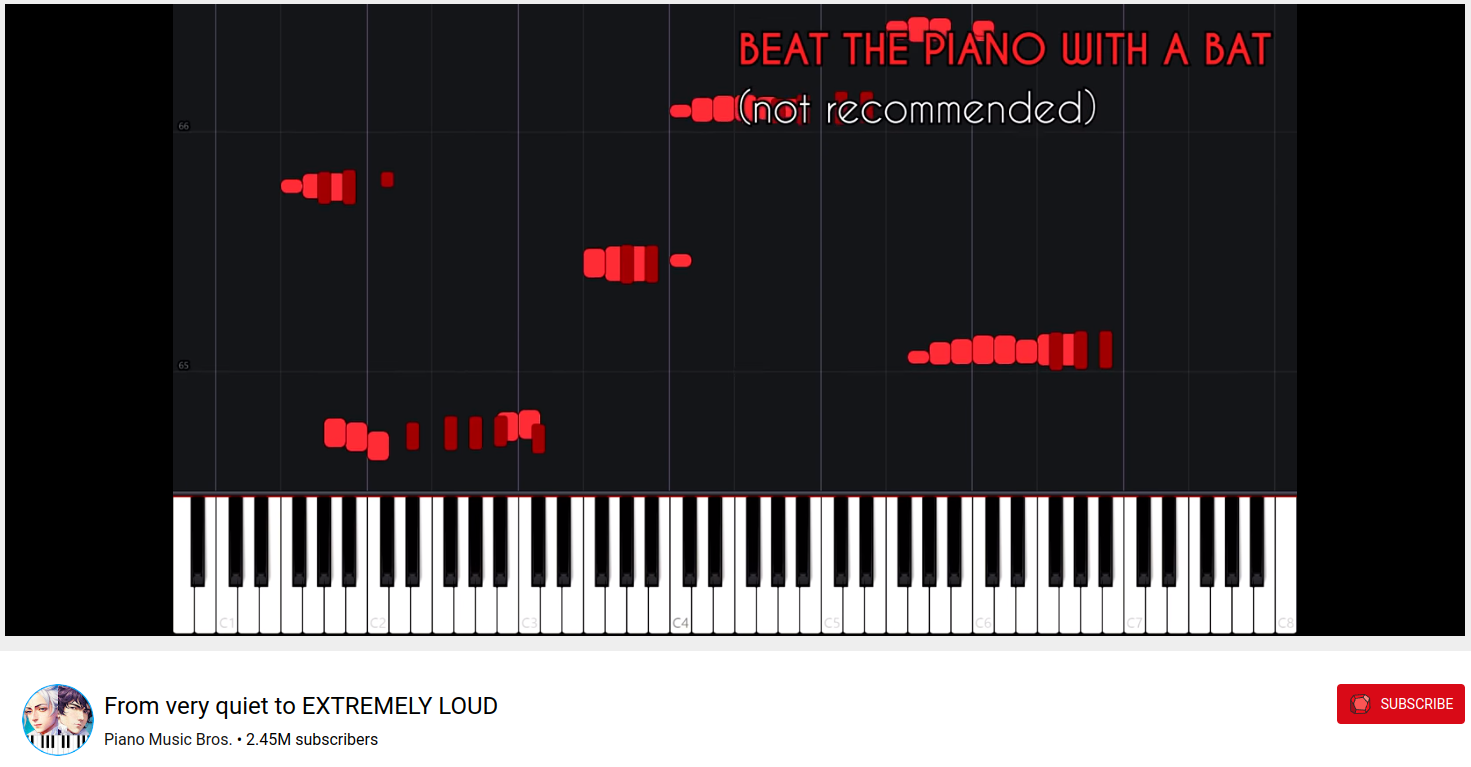
\includegraphics[width=0.6\columnwidth]{figures/malicious_audio.png}
%     \caption{A sample video which includes fast and loud piano notes. Usually in such videos, there is high tempo, no rhythm and varying pitches. The video also includes bright and striking hues, and also suggests a violent action of "hitting the piano with a bat"!}
%     \label{fig:ytkpiano}
% \end{figure}




\begin{figure}[!htb]
  \centering

  \begin{subfigure}{0.45\textwidth}
    \centering
    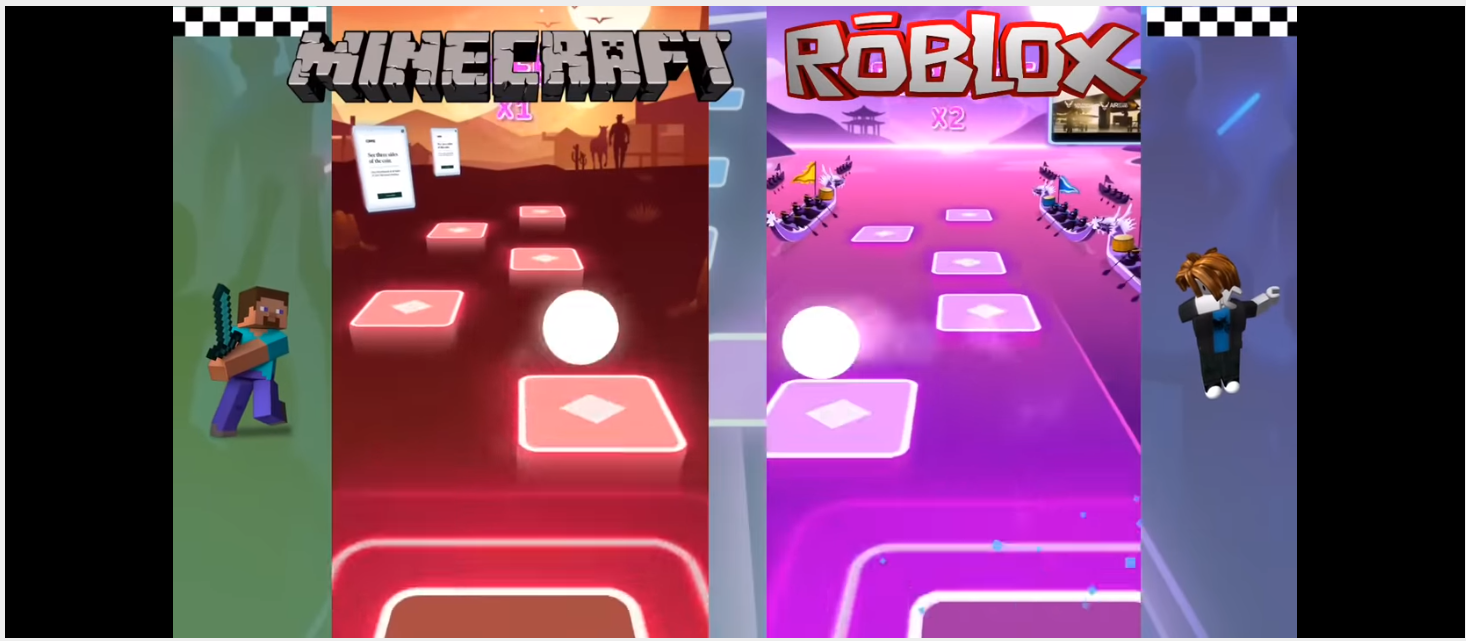
\includegraphics[width=\textwidth]{figures/malicious7.png}
    \caption{}
    \label{fig:image_a}
  \end{subfigure}
  \hfill
  \begin{subfigure}{0.45\textwidth}
    \centering
    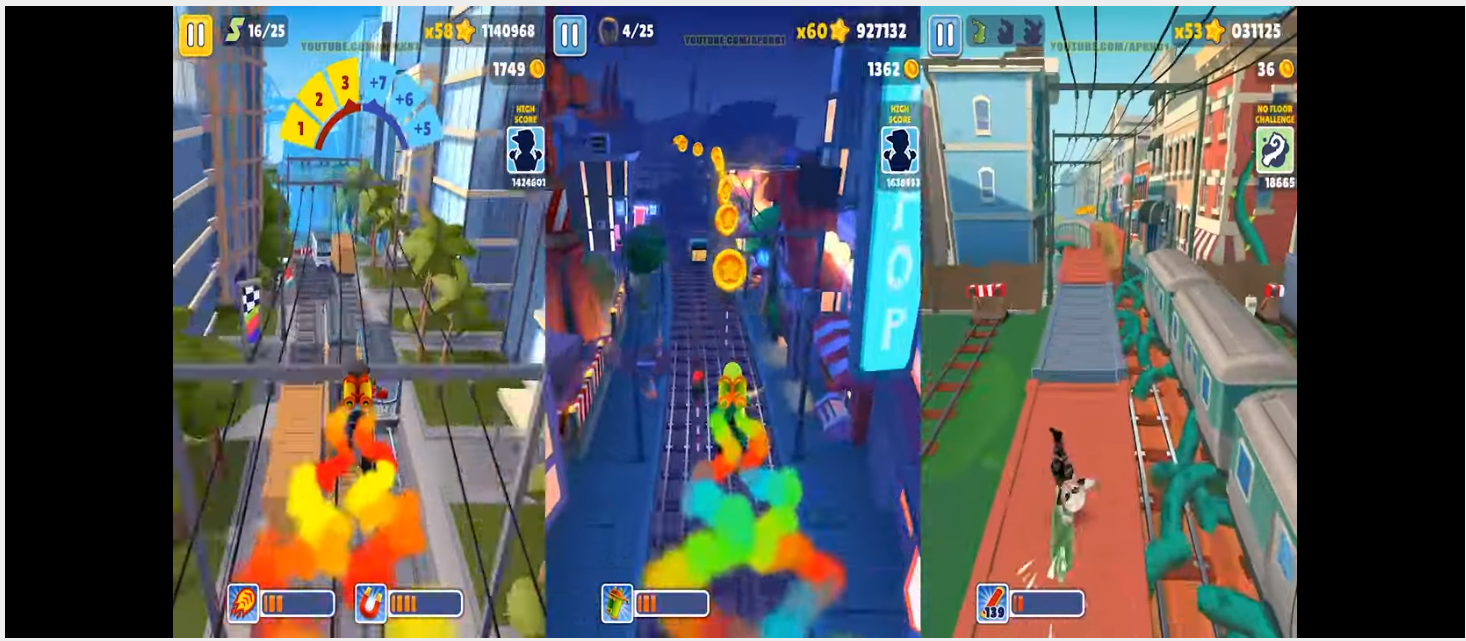
\includegraphics[width=\textwidth]{figures/malicious8.png}
    \caption{}
    \label{fig:image_b}
  \end{subfigure}

  \caption{a) shows a gameplay having striking colors which includes 2 different animations in 2 halves of the screen. b) shows a sample gameplay video for the Subway Surfer game displayed in a split-screen layout.}
  \label{fig:group_of_images}
\end{figure}

\begin{figure}[!htb]
  \centering

  \begin{subfigure}{0.45\textwidth}
    \centering
    
\includegraphics[width=0.8\textwidth]{figures/malicious5.png}
    \caption{}
    \label{fig:image_disgust}
  \end{subfigure}
  \hfill
  \begin{subfigure}{0.45\textwidth}
    \centering
    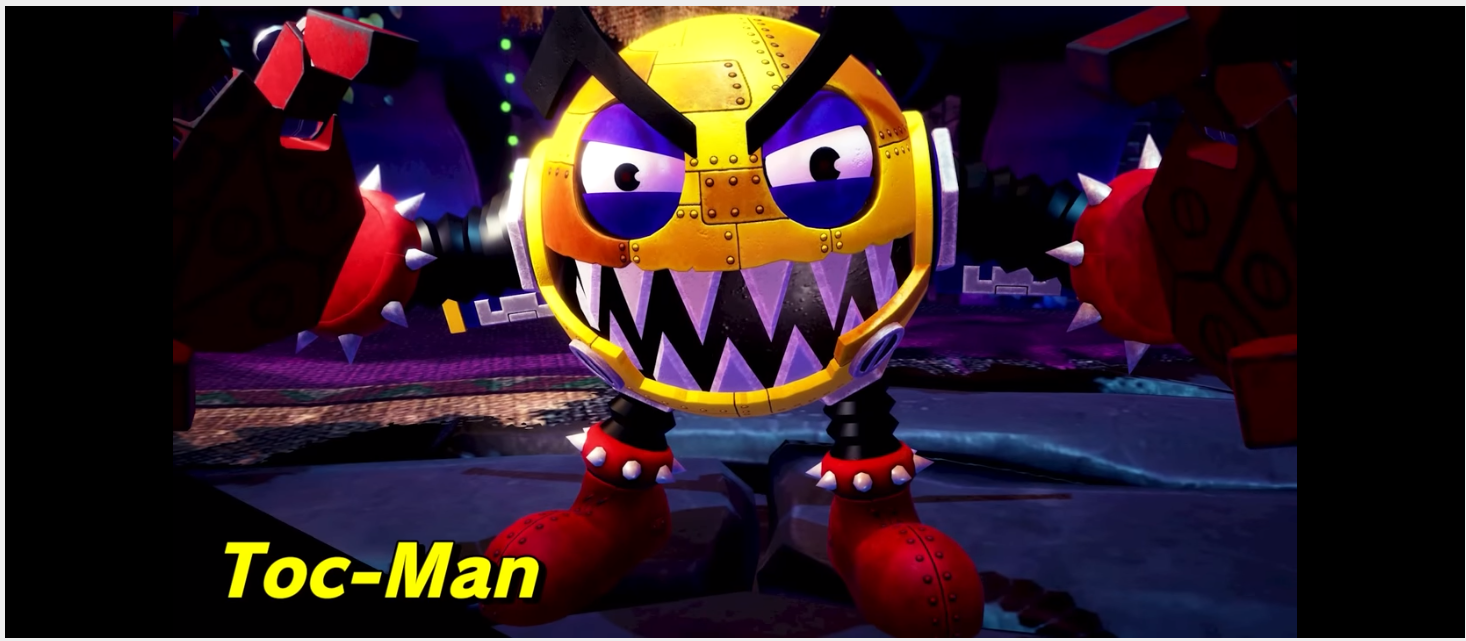
\includegraphics[width=\textwidth]{figures/malicious9.png}
    \caption{}
    \label{fig:image_angry}
  \end{subfigure}

  \caption{a) shows a disgusting and scary character b) shows a furious and frightening PacMan.}
  \label{fig:disgusting}
\end{figure}

\begin{figure*}[!h]
    \centering
    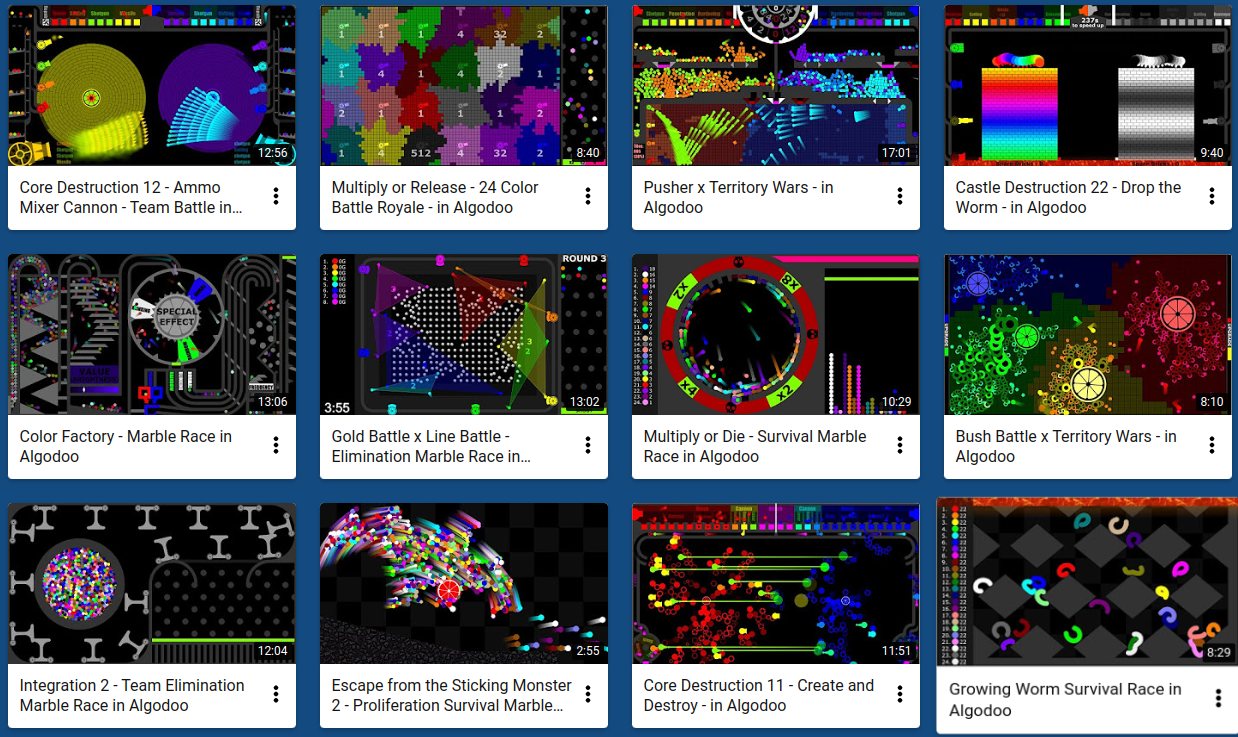
\includegraphics[width=0.8\textwidth]{figures/maliciou3.png}
    \caption{Videos of animations on YouTube Kids which include tiny fast-moving objects with bright colors.  The music soundtrack includes heavy metal and rock music.}  
    \label{fig:model}
\end{figure*}


% \begingroup
% \renewcommand{\arraystretch}{1.6}
% \begin{table}[h]
% \centering
% \begin{tabularx}{0.45\textwidth} { 
%   >{\raggedright\arraybackslash}X 
%   | >{\centering\arraybackslash}X 
%   | >{\centering\arraybackslash}X 
%   | >{\centering\arraybackslash}X
%   | >{\centering\arraybackslash}X 
%   | >{\centering\arraybackslash}X}
 
%  \textbf{Model} & \textbf{Layers} & \textbf{Patch Size} & \textbf{MLP Dim} & \textbf{Heads} & \textbf{Param} \\
%  \hline
%  \hline
%  ViT-B/16 & 12 & 16 & 3072 & 12 & 86M\\
%  ViT-B/32 & 12 & 32 & 3072 & 12 & 86M\\
%  % ViT-L/14 & 24 & 1024 & 4096 & 16 & 307M\\
% \end{tabularx}
% \caption{Comparison of CLIP base models.}
% \label{table:modelcomp}
% \end{table}
% \endgroup

\end{document}
